\documentclass[aps,prl,reprint,amsmath,amssymb,nature]{revtex4-1}

% define variable that compiles the main text (as opposed to SI text)
\newcommand*{\MAINTEXT}{}

\usepackage{epsfig,color,graphicx}

\begin{document}
\newcommand{\Ang}{\ensuremath{\mathring{\text{A}}}}
\newcommand{\ltwid}{\mathrel{\raise.3ex\hbox{$<$\kern-.75em\lower1ex\hbox{$\sim$}}}}
\newcommand{\gtwid}{\mathrel{\raise.3ex\hbox{$>$\kern-.75em\lower1ex\hbox{$\sim$}}}}
\newcommand{\bra}{\langle}
\newcommand{\ket}{\rangle}
%\newcommand{\sill}{\psi_\mathrm{SILL}}
\newcommand{\sill}{\psi}
\newcommand{\trace}{{\rm Tr}}
\newcommand{\ntilde}{\tilde{n}}
\newcommand{\stilde}{\tilde{s}}
\newcommand{\atilde}{\tilde{\alpha}}
\newcommand{\new}{\color{red}}
\newcommand{\blue}{\color{blue}}
\newcommand{\old}{\color{black}}
\newcommand{\bea}{\begin{eqnarray}}
\newcommand{\eea}{\end{eqnarray}}
%\newcommand{\bea}{\begin{equation} \begin{split}}
%\newcommand{\eea}{\end{split} \end{equation}}
\def\nn{\nonumber\\}

\bibliographystyle{naturemag}

%\ifdefined\MAINTEXT
%\else
%	\clearpage
%	%\widetext
%	\setcounter{figure}{0}
%	\setcounter{page}{1}
%	\renewcommand{\thefigure}{S\arabic{figure}}
%\fi

\title{
\ifdefined\MAINTEXT
\else
Supplementary Information: \\
\fi
Contribution of the covalent component of the hydrogen-bond network to the properties of liquid water
}

\author{Yifei Shi}
\author{Hayden Scheiber}
\author{Rustam Z. Khaliullin}
\email{rustam.khaliullin@mcgill.ca}
\affiliation{Department of Chemistry, McGill University, 801 Sherbrooke St. West, Montreal, QC H3A 0B8, Canada}

\date{\today}

\ifdefined\MAINTEXT

\begin{abstract}
Many remarkable properties of liquid water originate from the ability of its molecules to form hydrogen bonds, each of which emerges as an intertwined combination of electrostatic, polarization, dispersion, and donor-acceptor or covalent interactions.
%each of which is a combination of electrostatic, polarization, dispersion, and covalent interactions. 
In this work, \emph{ab initio} molecular dynamics is tuned to disentangle and switch off the covalent component of interactions between water molecules in simulations. 
Comparison of simulations with and without covalency shows that a small amount of intermolecular electron transfer has a profound effect on the structure and dynamics of the hydrogen-bond network and thus on observable properties of room-temperature liquid water. 
The findings of this study do not only deepen our knowledge about the fundamental nature of hydrogen bonding, but can also aid interpretation of spectroscopic response, catalytic behavior, and solvation properties of aqueous systems.
\end{abstract}

\maketitle

%RZK0: em dashes, HBs - double meaning

\section{Introduction} 

Detailed understanding of the physical nature of hydrogen bonding (HB) between molecules in water is essential for unraveling the origins of the unique physical and chemical properties of this ubiquitous and important liquid. 
Since the dawn of quantum mechanics, it has been known that HB is a complex phenomenon that arises from the interplay of several distinct effects: interaction between molecules' permanent multipoles (dipoles, quadrupoles, etc.), polarization, dispersion, and orbital donor-acceptor interactions~\cite{eisenberg2005structure}.

Donor-acceptor interaction leads to the transfer of electron density between molecules and is therefore known as the charge-transfer or covalent component of HB. 
The concept of covalent interaction in HB is tremendously useful in chemistry, as
%[and is deeply embedded into the everyday chemistry jargon/language. It helps] 
it helps to explain water's unique properties as a solvent as well as its ability to catalyze a wide variety of chemical processes. Covalent interaction also helps to explain the strong cooperativity between hydrogen bonds in systems ranging from nanodroplets to solvated biomolecules. 
From a theoretical standpoint, the covalent component of HB has attracted significant attention because of its purely quantum mechanical nature, which---unlike electrostatic and dispersion interactions---is difficult to describe with simple analytical potentials~\cite{lee2011effects, gordon2013accurate}.



Recent developments in energy decomposition techniques based on accurate electronic structure methods have helped make substantial progress towards quantifying the individual contributions of various physical effects on the HB energy in small water clusters. 
However, the extent of intermolecular charge transfer in HB has remained the last unresolved issue until recently~\cite{isaacs1999covalency,ghanty2000hydrogen,stone2017natural}. 
Natural bond orbital analysis~\cite{weinhold1998natural} and natural energy decomposition analysis \cite{glendening1994natural} have suggested that charge transfer is the major component of HB~\cite{schenter1996natural,glendening2005natural,weinhold2005resonance} because---when charge transfer is neglected---these methods yield no binding at the water-dimer equilibrium geometry. 
After a debate spanning several decades, it has been argued that natural bond orbital analysis is not optimal for weak interactions~\cite{stone2017natural}.
It appears that the covalent component of HB is better described by early decomposition methods~\cite{kitaura1976new,bagus1984new,bagus1992decomposition,stevens1987frozen,chen1996energy,stone1993computation} as well as their modern variants~\cite{mo2000energy,misquitta2013charge,khaliullin2007unravelling,misquitta2013charge}. 
According to these methods, charge transfer contributes only around 20--30\% of the overall binding energy between water molecules in small clusters \cite{stevens1987frozen,stone1993computation,chen1996energy,piquemal2005csov,khaliullin2009electron,cobar2012examination}, in agreement with many chemists' long-held intuitive view of HB.

%RZK0 this is QAIM: Grabowski2011 - 10.1021/cr800346f

While energy decomposition methods have helped us understand the importance of charge-transfer in the binding strength of gas-phase water clusters, nothing is known about the covalent contribution of HB to the \emph{observed} properties of liquid water. 
A deep connection between the covalent interactions and features of the X-ray absorption~\cite{NatureComm2013}, infrared~\cite{JPCL2013}, and nuclear magnetic resonance~\cite{NatureComm2015} spectra of liquid water has been pointed out in several recent articles. 
In this work, we extended a recently developed energy decomposition method for periodic systems~\cite{Khaliullin2013JCTC} to perform an unprecedented \emph{ab initio} molecular dynamics study that measures quantitatively the contribution of the covalent component of HB to the structural, dynamical, and spectroscopic properties of liquid water in ambient conditions. 
Our results show that the seemingly insignificant covalent component of HB is a defining feature in many properties of liquid water. 
%[has a profound effect on the properties of water].


%In this work, we combined \emph{ab initio} molecular dynamics with a recently developed energy decomposition method for periodic systems~\cite{Khaliullin2013JCTC} to perform an unprecedented computational study that measures quantitatively the contribution of the covalent component of HB to the structural, dynamical and spectroscopic properties of liquid water at ambient conditions. 

\section{Methodology}

To quantify the influence of the covalent component of HB on the observed properties of liquid water, we compared the properties calculated with \emph{ab initio} molecular dynamics (AIMD) using two different models. 
One model incorporates the intermolecular covalency fully whereas the other removes it completely.

The first model is the conventional Kohn-Sham density functional theory (DFT) approach, in which the electrons of a water molecule are delocalized over all neighbors. 
This model is known to reproduce properties of liquid water reliably, in semi-quantitative agreement with experimental measurements. 
%The quality of the simulations was verified by comparing the results to the experimentally available data. 
In this work, the first model is referred to as the delocalized-electron, reference, or realistic model. 
% Agreement is semiquantitative

The second model is a constrained DFT method based on absolutely localized molecular orbitals (ALMO)~\cite{khaliullin2006efficient}. 
Unlike conventional DFT, ALMO DFT~\cite{Khaliullin2013JCTC} is able to confine each electron strictly to its own molecule and therefore completely remove the covalent component from intermolecular bonding. 
Mathematically, this is achieved by expanding Kohn-Sham molecular orbitals \emph{only} in terms of the atomic orbitals of the parent molecule~\cite{stoll1980use,khaliullin2006efficient, mo2000energy}.
Such molecular orbitals are called absolutely localized because they are localized on molecules, in the same sense as atomic orbitals are localized on atoms. 
In the interest of brevity, intermolecular interaction without covalent component will be referred to as \emph{devalent} interactions and the ALMO-based model will be called the localized-electron or the \emph{devalent} model. 
It is important to note that the devalent model retains all other physical effects, including the covalent component of \emph{intramolecular} OH bonds. %were variationally optimized on each AIMD each step to find the electronic ground state of the system.
Theoretical methods that ensure the covalent component of intermolecular bonding is removed accurately are described in Computational Methods, together with pertinent accuracy tests.

To keep electrons absolutely localized over the course of AIMD simulations, we extended the recently developed ALMO DFT method for condensed molecular systems~\cite{Khaliullin2013JCTC} so that the atomic forces can be computed analytically from the ALMO DFT energies (see Computational Methods).

All AIMD simulations---with either delocalized or localized molecular orbitals---were performed using the dispersion-corrected~\cite{grimme2010consistent} BLYP exchange-correlation functional~\cite{becke1988density, lee1988development} and the TZV2P basis set~\cite{vandevondele2007gaussian}. 
The temperature of simulations was set to 298~K. 
The size of the periodic cubic simulation box was fixed to reproduce the experimental 0.997~g$\cdot$cm$^{-3}$ density of ambient liquid water. 
Since removing intermolecular covalency can affect the density, we also performed a set of simulations for a system in which density was adjusted to 1~atm using constant pressure AIMD. 
The length of the AIMD simulations were chosen to obtain statistically meaningful results. 
A detailed description of the calculations is presented in Computational Methods.

It is important to comment on the ability of the reference model to reproduce properties of real water. 
The accuracy of the model is mostly determined by the ability of the exchange-correlation functional to reproduce the energetics of intermolecular interactions. Like many generalized gradient approximation functionals, BLYP is known to underestimate the energy gap of molecules slightly. 
Because of this, the strength of intermolecular binding is overestimated and any computed radial distribution functions have slightly sharper peaks than those derived from X-ray scattering experiments. 
The overbinding effect also results in an underestimated diffusion constant and overestimated viscosity. 
Nevertheless, it is shown below that almost all properties of liquid water calculated with the BLYP exchange-correlation functional are in semi-quantitative agreement with experimental data. 
Moreover, for all calculated properties the imperfections in the reference model are far less significant than the changes induced by neglecting intermolecular covalency. 
That is why the devalent model in this work provides a reasonable semi-quantitative estimate of the contribution of the covalent component of intermolecular bonding on the observed properties of liquid water.


\section{Results and discussion}

The variational principle of quantum mechanics guarantees that removing covalent interactions can only weaken intermolecular bonding. 
ALMO-based decomposition energy analysis predicts that---in a water dimer---the transfer of 0.27\% of an electron contributes  7.0~kJ$\cdot$mol$^{-1}$ (37\%) to the overall stabilization of the hydrogen bond at equilibrium geometry, in agreement with earlier reports~\cite{stevens1987frozen,chen1996energy,piquemal2005csov,khaliullin2009electron}. 

This contribution is higher in the \emph{cooperative} HB network of liquid water at ambient conditions: 1.1\% of an electron and 19 ~kJ$\cdot$mol$^{-1}$ per hydrogen bond, in agreement with our previous study \cite{kuhne2014nature}.

\begin{figure}
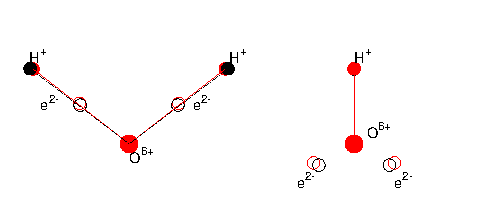
\includegraphics[width=0.5\textwidth]{acoord}
\caption{Average positions of atoms (solid circles) and Wannier centers (empty circles) in a water molecule for the realistic (black) and devalent (red) models. 
} \label{Fig:acoord}
\end{figure}

\textbf{Molecular structure.} The covalent component of weak intermolecular bonds has only a minor effect on the shape of water molecules (Figure~\ref{Fig:acoord}). 
The average length of intramolecular OH bonds changes from 0.992~\Ang\ in the realistic model to 0.977~\Ang\ in the devalent model of water. 
At the same time, the average intramolecular HOH angle changes from 105.5 degrees to 104.3 degrees, becoming closer to the value calculated for 298~K gas phase water molecules.

\begin{figure}
%HOS: "A" and "B" labels not present in these plots
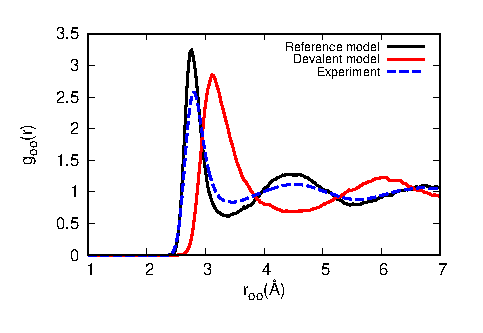
\includegraphics[width=0.5\textwidth]{new_rdf}
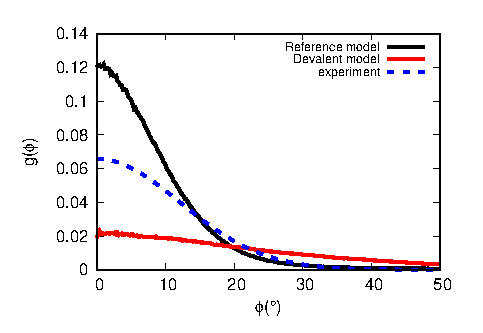
\includegraphics[width=0.5\textwidth]{new_adf}
\caption{A. Oxygen-oxygen radial distribution function. B. Distribution of HB angles $\phi \equiv O_{\text{ref}} \cdots O-H$ computed for hydrogens within 2.3~\Ang\ from a reference atom. The angular distribution function is normalized to account for the $\phi$-dependent volume and to correctly emphasize the energetic preference for linear HBs (see Supplementary Information). The experimental curve is taken from Ref.~\onlinecite{modig2003temperature}.} \label{Fig:RDF}
\end{figure}

%RZK0: Suggested color coding throughout the manuscript: realistic - black, devalent - red, experiment - black dash, vapor - blue, devalent NPT - blue (these colors make it easier for color blind persons to read figures and at the same time minimize the publication cost). Legends throughout: ``Realistic model'', ``Devalent model'', ``Experiment''. 

The effect of covalency on the structure of the HB network is far more pronounced than other structural properties. 
The oxygen-oxygen radial distribution function (RDF) in Figure~\ref{Fig:RDF}A shows that weaker devalent interactions lead to a considerable expansion in the first coordination shell of water molecules from the ``realistic'' average of 2.8~\Ang\ to 3.1~\Ang. 
The shift of the first-shell peak is accompanied by broadening that is indicative of a wider variety of configurations available to devalent HBs.

These dramatic changes in the structure of the HB network are consistent with the decrease in HB strength. 
It is remarkable, however, that the remaining components of HB---permanent electrostatic, polarization, and dispersion interactions---are sufficiently strong to retain several characteristic structural features of the network, including well-defined coordination shells and directional HBs~\cite{arunan2011definition}.
Indeed, the second coordination peak in the RDF of the devalent model remains clearly visible though shifted to higher distances. 
The distribution of HB angles also retains a maximum at 0$^\circ$ despite becoming significantly broader (Figure~\ref{Fig:RDF}B).

The structure of the HB network for both models can also be illustrated with the spatial distribution of oxygen atoms around a reference water molecule (see cross sections in Figure~\ref{Fig:SDF}). 
It is clear that the distorted tetrahedral structure of liquid water is retained without the covalent component (cf. Figure~\ref{Fig:SDF}A and \ref{Fig:SDF}AB), indicating that permanent electrostatic and polarization interactions tend to orient water molecules the same way as covalent interactions. 
For comparison, if a model retains only dispersion interactions and short-distance repulsion, represented by the Lennard-Jones potential, the HB becomes truly non-directional with uniform angular distribution (Figure~\ref{Fig:SDF}C). 
This is why permanent electrostatics is widely recognized as the key component of interaction between water molecules and is included in all analytical molecular mechanics models of water. 
On the other hand, the equally strong covalent component is neglected in these models and instead compensated for by fine-tuning permanent atomic charges (see Figure~\ref{Fig:SDF}D, for example). 

\begin{figure}
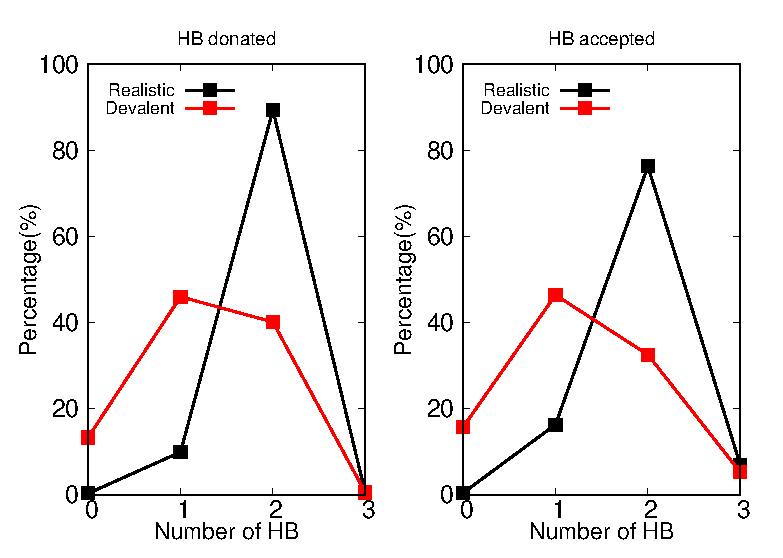
\includegraphics[width=0.4\textwidth]{new_hbstat}
%HOS: Increase text size to match figure 2?
\caption{HB statistics for liquid water with and without intermolecular covalency.}\label{fig:HBstat}
\end{figure}

\begin{figure*}
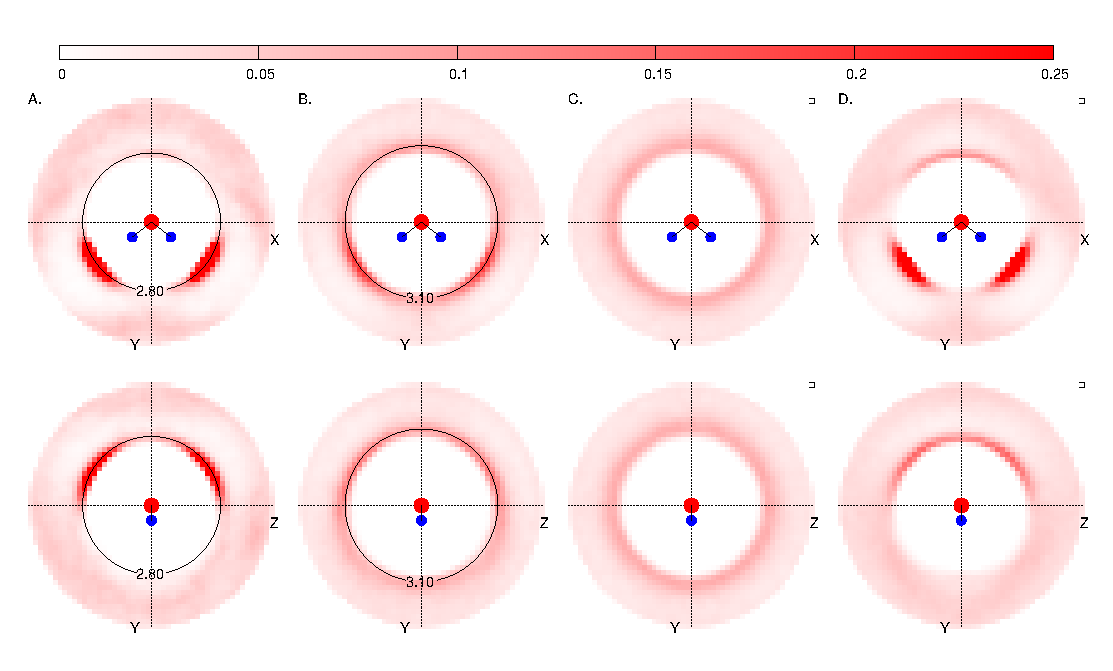
\includegraphics[width=0.9\textwidth]{SDF}
\caption{Cross sections of the spacial distribution of oxygen atoms. 
The upper panels show the cross section of the spacial distribution function in the plane of the reference water molecule, whereas the lower panels show the cross section in the plane bisecting the molecule. 
A. Reference model, B. localized model, C. Modified TIP3P model that includes only van der Waals interactions, D. TIP3P model: electrostatic interactions between atomic point charges combined with van der Waals interactions~\cite{TIP3P}.} \label{Fig:SDF}
\end{figure*}

%"It is interesting that the average intermolecular distance increases significantly when covalent component is switched off (Figure~\ref{Fig:RDF}A) while the density of both reference and devalent models is fixed to be the same. This indicates that" 
%Note: This statement might not be entirely correct. A better statement is that the position of the first coordination peak shifts to higher distance. The total average number of molecules around a reference molecule within the shpere of radius R is given by the integral of the RDF from zero to R in the spherical coordinates. The R-dependent integrals can have different values depending on how molecules are distributed. Computing them can explain the shift in the first peak at the fixed density. Both integrals will converge to the same value for the reference and devalent models at large enough R because the density is the same.

%\Yifei: I did the integral, they are close, but not exactly the same, maybe due to finite width of the bins.  
% When the cut off is half the system size, the integral for realistic model: 212, devalent: 209. 
% RZK: The values are close enough to each other. Did you take into account the 4 \pi r^2 factor during the integration? I assume that the total number of molecules in the cell is 125. At half-size the integral must be less than 125 (unaccounted oxygen atoms in the corners of the cubic cell), not more than 125.
%\Yifei: I was not sure how the rdf is normalized, and tried both with and without the r^2 factor. The previous one was without the factor, with the factor, realistic 721, devalent 713. 
 
\textbf{HB statistics.} The drastic difference in the structure of the HB network of the realistic and devalent models is confirmed by analysis of the HB statistics. 
The commonly accepted---though somewhat arbitrary---binary geometric definition of a HB is utilized: the H--O$\cdots$O angle must be smaller than 30$^{\circ}$ and the O-O distance must be shorter than 3.5\Ang~\cite{rey2002hydrogen,lawrence2003vibrational}. 
The distribution of molecules according to the number of donated or accepted HBs in Figure~\ref{fig:HBstat} shows that switching off intermolecular covalency leads to an increase of single-donor and single-acceptor molecules. 
The increase is so drastic that single-donor and single-acceptor molecules outnumber those with two HBs.
In total, there are 35\% fewer HBs in the devalent than in the reference model of water.

\textbf{Density.} If the density is allowed to fluctuate in a simulation while the pressure is fixed at 1~atm, the average density decreases from 0.99~g$\cdot$cm$^{-3}$ for the reference model to 0.85~g$\cdot$cm$^{-3}$ for the devalent model, a decrease of 14\%. 
While this is a noticeable drop, it is important to note that the devalent water is still liquid at ambient conditions because of the strong electrostatic, polarization, and dispersion effects. 

The 14\% decrease in density should correspond to a 5\% elongation in intermolecular distances, assuming a uniform increase among molecules. Nevertheless, the position of peaks in the RDF remains unchanged in the devalent water at the two different densities (Figure~\ref{Fig:rdf_cp} in Supplementary Information). The only noticeable structural changes are that peaks in the RDF become slightly broader in the low-density constant-pressure model (Figure~\ref{Fig:rdf_cp}), and the angular distribution is more narrow (Figure~\ref{Fig:ir_cp}). This indicates that most molecules stay in the same position around the minimum of the potential well when the density is allowed to relax. Only a small fraction of them become distorted radially or angularly. 

We will continue discussing properties of the \emph{fixed-density} devalent water further because all key properties obtained for the \emph{fixed-pressure} model are almost the same, while calculations are more difficult for the latter (see Supplementary Information).

% density of butanol is 0.810, 3-Pentanone -- 0.815, 2-Octanol -- 0.824

\textbf{Infared spectrum.} Figure~\ref{Fig:IR} shows the infared (IR) spectra of the devalent and reference systems together with that of ideal water vapor at 298~K. The spectra are calculated entirely from the time-dependent positions of atoms and Wannier centers (Figure~\ref{Fig:acoord}) as described in Ref.~\onlinecite{thomas2013computing}.

The most pronounced difference between the IR spectra is in the 3000--4000~cm$^{-1}$ region of intramolecular O--H stretching band $\nu_s$. 
For the devalent model, the $\nu_s$ peak does not exhibit the redshift and broadening characteristic to hydrogen-bonded O--H groups clearly seen in the spectrum of the realistic model. 
Comparison between the spectra of the devalent and gas-phase models indicates that the characteristic redshift is entirely due to intermolecular covalent interactions. 
Apparently, even the small amount of electron density transferred to the antibonding orbitals of intramolecular O--H bonds (see Figure~2 in Ref.~\onlinecite{khaliullin2009electron}) is sufficient to ``soften'' the O--H bond and lower its vibrational frequency by 600~cm$^{-1}$.

The primary role of the covalent component in the broadening of the $\nu_s$ peak is also apparent from Figure~\ref{Fig:IR}. 
The broadening of $\nu_s$ is normally attributed to a great variation in the strength of HBs in liquid water, with stronger HBs leading to redshifts of larger magnitude. 
As discussed above, devalent water exhibits greater variation in the geometry of HB structures than the realistic model (compare Figure~\ref{Fig:RDF}A and~\ref{Fig:SDF}A-B). 
Despite this increased variety, the $\nu_s$ peak of devalent water remains very narrow. This fact confirms that a HB without the covalent component does not generate a significant redshift. 
%that the symmetric and asymmetric stretching modes become resolved in the spectrum of devalent model?

%Yifei: The integrated intensity is discussed in Eq 5.1 of the book "The HB and the water molecule".

Finally, a comparison of the stretching bands for the three models shows that the spectacular enhancement of the integrated intensity from the gas to the liquid phase is not entirely due to the intermolecular electron transfer as was previously assumed~(see Chapter 5 in Ref.~\onlinecite{marechal2006hydrogen}). 
It is well known that the integrated intensity is proportional to $\left({\partial \mu}/{\partial q}\right)^2$---the derivative of the dipole moment with respect to the coordinate of the vibrational mode (i.e. the intramolecular O--H distance)---and any change in the integrated intensity arises mostly from the change in this derivative. 
The change in this derivative is attributed to decoupling of the motion of electrons from that of the nuclei in HB systems: stretching of a hydrogen bonded O--H group causes the electrons (i.e. Wannier centers in Figure~\ref{Fig:acoord}) not to follow the H-atom as closely as when no HB is established~\cite{marechal2006hydrogen}. 
Our data shows that the derivative changes both from the gas-phase to the devalent model and from the devalent to the realistic model. 
This means that the mere presence of a neighbor's lone pairs leads to decoupling, while the intermolecular electron transfer makes this effect more pronounced.

%\[ M_0 \propto \left( \frac{\partial \mu}{\partial q} \right)^{2} \vert \langle 0 \vert q-q_0 \vert 1 \rangle \vert ^{2}
%\]
%%
%where $q$ is the distance between H and Y in a X-H...Y bond, $q_0$ is the equilibrium position, $\mu$ is the dipole of the X-H...Y systems. $\vert \langle 0 \vert q-q_0 \vert 1 \rangle \vert \sim h\omega/2$ for harmonic osillator and doesn't change much. So the change is mainly from $\frac{\partial \mu}{\partial q}$, which means that in the realistic model when stretching the X-H bond electron won't follow the H atom as much, or in the realistic model the electron are more detatched to the H atoms than the devalent model, due to electron transfer.

Unlike stretching modes, the intramolecular bending modes in the region of 1600~cm$^{-1}$ are unaffected by intermolecular forces and remain approximately the same for the realistic, devalent, and ideal-gas systems. 
It is worth noticing that the stretching and bending peaks of the devalent model do not exhibit the extensive rotational structure---visible in the spectra of gas-phase molecules---because the retained intermolecular forces are sufficiently strong to hinder rotations.

Another significant difference between the realistic and devalent systems is in the peaks below 1000~cm$^{-1}$, which correspond to HB stretching vibrations and molecular librations ($\sim$200~cm$^{-1}$ and $\sim$700~cm$^{-1}$ in the realistic model, respectively). These peaks are shifted in the direction opposite to the intramolecular stretching modes. This is because intermolecular bonding---unlike intramolecular bonding---becomes softer when the covalent component of the interaction is switched off, in agreement with the observed variety of geometric configurations accessible in the devalent water. 

\begin{figure}
\centering
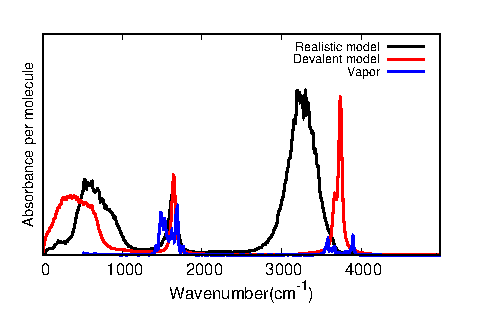
\includegraphics[width=0.5\textwidth]{new_ir}
\caption{Calculated IR spectra. The far infrared part of the spectrum for the ideal-gas system, which corresponds to rotational modes, is removed for clarity. 
} \label{Fig:IR}
\end{figure}

\textbf{Molecular dipole moment and dielectric constant.} Water's unique properties as a solvent are due to both the high dipole moment of its molecules and its high dielectric constant. 
The latter accounts for the ability of the molecular dipoles to reorient, as well as to stabilize ions and polar solute molecules. 

Molecular dipole moments in condensed phases cannot be defined unambiguously, because there is not a unique way to assign a continuous electron density to molecules.
Here, we utilized a standard procedure that estimates molecular dipoles using the positions of the centers of maximally localized Wannier orbitals (Figure~\ref{Fig:acoord})~\cite{marzari1997maximally,sharma2007dipolar}. 
The resulting distribution of molecular dipoles in shown in Figure~\ref{Fig:dipoledist}.  
The calculated average dipole moment of water molecules are 3.09~D for the reference model, or 1.96~D for an isolated molecule at 298~K.
These values are in good agreement with the experimentally measured 2.9$\pm$0.6~D~\cite{badyal2000electron} and 1.85~D~\cite{haynes2014crc} dipole moments, respectively. 
For comparison, the average dipole moment of molecules in the devalent system is 2.47~D indicating that covalent interactions are only partially responsible for the impressive $\sim$1~D increase in the molecular dipole moment from the gas to condensed phase. 
Figure~\ref{Fig:acoord} shows that the change in the dipole moment is caused primarily by the change in the position of lone electron pairs on the oxygen atom. 
At the same time, the wider spread of dipole moments in the realistic model (Figure~\ref{Fig:dipoledist}) is attributable to the four-fold increase in the spread of positions of electron lone pair centers. 
To be precise, intermolecular charge transfer increases the standard deviation from the average position of the lone pair centers from 0.07~pm in the devalent model to 0.29~pm in the realistic model.
%
%Yifei: The standard deviation of positions of atoms in Angstrom: 
% Realist: H 0.0045 WC(top) 0.0016 WC(bottom) 0.0029
% Devalent: H 0.0032 WC(top) 0.0011 WC(bottom) 0.0007

\begin{figure}
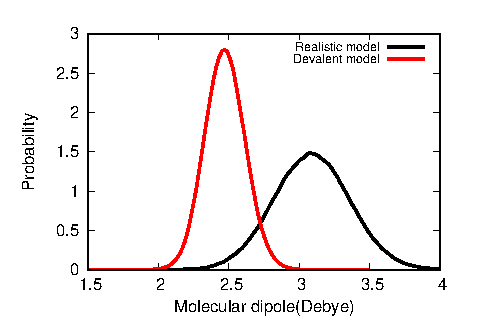
\includegraphics[width=0.45\textwidth]{new_dipole}
\caption{Distribution of dipole moments of water molecules.} \label{Fig:dipoledist}
\end{figure}

The dielectric constant can be calculated using the fluctuation of the total dipole moment of the system~\cite{neumann1983dipole,adams1981theory}:
%
\bea
\epsilon = 1+\frac{4\pi}{3V k_B T}  (  \langle |\vec{M}|^2 \rangle  - \langle |\vec{M}| \rangle ^2) \label{Eq:dielectric}
\eea
%
where $V$ and $\vec{M}$ are the volume and total dipole of the simulation box, respectively. 
While the dielectric constant for the realistic model is 70---in good agreement with the experimental value of 78---this value increases to a remarkable 180 for the devalent model.
We attribute this dramatic increase to the facile reorientation and greater mobility of molecules in the devalent model, which are not held as strongly by the weakened HBs. 
Thus despite its smaller molecular dipoles, devalent water would be a solvent of unprecedented strength for dissolving polar solutes.

\textbf{HB dynamics, diffusion, and viscosity.} In order to describe the influence of intermolecular covalency on the dynamics of the HB network, the HB lifetime $\tau_{\text{HB}}$ was calculated from the \emph{continuous} HB time autocorrelation function as described in the Supplementary Information. The lifetime obtained from the continuous autocorrelation function measures the ability of a HB to survive without being broken---even fleetingly.

The 0.7~ps HB lifetime calculated for the realsitic model agrees well with experimental estimates \cite{lawrence2003ultrafast} and previous simulations~\cite{marti1996molecular,starr1999fast}. Removing intermolecular covalency shortens the HB lifetime substantially, almost by an order of magnitude, to 0.08~ps. 

%The reference lifetime does not seem to agree with previous calculations (e.g. doi:10.1039/c3cp51039e). Is it because of the different definition of $C_{\text{HB}}(\tau)$ or because of the simple single-exponent model? In any case, we need convincing evidence that our $\tau=0.7$~ps is reliable. \old One order of magnitude difference in the HB lifetime indicates that by strengthening HBs covalent interactions also increase energetic barriers on the pathway of their breaking-formation process.
%Yifei: There are different ways to define the HB life time. See https://doi.org/10.1016/S0009-2614(02)02039-0   
%I'm using similar definition, and the result seems to agree with experiment \cite{lawrence2003ultrafast} and MD %\cite{marti1996molecular,starr1999fast}.

The importance of covalent interactions in HB dynamics is also reflected by its influence on the self-diffusion coefficient and shear viscosity. 
Here, both of these quantities are calculated using the method of D\"unweg and Kremer~\cite{dunweg1993molecular}, which corrects for strong finite-size effects in the calculated quantities (see Supplementary Information). The results are listed in Table~\ref{Tab:dfs}. 
While the calculated reference values for the self-diffusion coefficient and shear viscosity are somewhat different from the experimental measured values, this is an expected consequence of the overestimated interaction strength in the XC functional (see Computational Methods). 
Despite this inaccuracy, it is clear that molecules in devalent water diffuse much faster and approximately 90\% of water's shear viscosity originates from covalent interactions between molecules.

\begin{table}
\caption{Diffusion, viscosity, and dielectric constants of liquid water at ambient conditions.}\label{Tab:dfs}
\begin{tabular}{l*{6}{c}r}
\hline
               & $D (\Ang^2/\text{ps})$ & $\eta (\text{Pa}\cdot \text{s})$ & $\epsilon$ \\
\hline
Devalent model                & 0.7188 & 3.5$\times 10^{-4}$ & 70 \\
%
Realistic model              & 0.1069 & 29.5$\times 10^{-4}$ & 180 \\
%
Experimental            & 0.239~\cite{hardy2001isotope}  & 8.9 $\times 10^{-4} $~\cite{harris2004temperature} & 78~\cite{haynes2014crc}
\end{tabular}
\end{table}
 
\section{Conclusions}

The amount of intermolecular electron density transfer in a typical HB of liquid water at ambient conditions is on the order of 1\% of an electron. 
However, this seemingly small covalent component has a profound effect on the strength and stability of individual HBs and---as a result---is responsible for a substantial change in the collective behavior of the HB network and observable properties of liquid water. 
Simulations show that removing covalency from intermolecular interactions shortens the lifetime of a HB by an order of magnitude and drastically increases the mobility of molecules. 
Without the covalent component, weaker HBs produce a liquid with significantly lower viscosity---comparable to that of acetone. 
The dipole moment of the average water molecule is only slightly lower if intermolecular charge transfer is forbidden, because electron pairs on oxygen atoms do not extend as far towards neighboring molecules. 
Despite this, the dielectric permittivity of devalent water is increased two-fold, mostly due to the ease reorientation for mobile molecules. 
In addition to providing a reasonable quantitative estimate of the contribution of the covalent component on the properties of water, our work reveals that intermolecular covalency is entirely responsible for the large redshift and broadening of the O-H stretching peaks in its IR spectra. It is only partially responsible for a dramatic increase in the intensity of these peaks. 

It is interesting to note that some properties of devalent water---with its weaker HBs---resemble those of real water at a higher temperature (e.g. diffusion coefficient, viscosity, and HB lifetime). 
This is to be expected because of the equivalence of energy and temperature in the Boltzmann factor. However many properties, such as the power spectrum and dielectric constant, respond to the removal of intermolecular covalency in a less intuitive way. 
For example, the dielectric constant of high-temperature real water is lower than that of room-temperature real water, whereas room-temperature devalent water has a much higher dielectric constant. 
This response originates from a nontrivial coupling of the covalent component of HBs to the other electronic degrees of freedom (e.g. intramoleclar position of the Wannier centers) and nuclear motion.

While the small covalent component of HBs strongly affect many properties of water, there are other intermolecular forces of different nature (frozen electrostatics, polarization, and dispersion) that strongly hold water molecules together. 
Our simulations show that, upon removal of the HB covalency, water remains liquid and maintains its structure and properties similar to those of real water. 
This result explains the success of empirical force fields that do not include small charge transfer explicitly, but instead artificially strengthen intermolecular interaction by increasing permanent atomic charges~\cite{rick2016polarizable}. 
While such simple empirical models reproduce a wide variety of properties in aqueous systems~\cite{vega2011simulating}, they will perform poorly for thermodynamic states of water with different amounts of intermolecular charge transfer (e.g. high-pressure water phases or aqueous interfaces with various materials). 
This is because the varying covalent interactions will not be fully compensated for by fixed empirical electrostatics.
Our data implies that even a small mismatch will lead to substantial errors in the properties obtained by using fixed empirical models.

To conclude, this work demonstrates that ALMO-based \emph{ab initio} molecular dynamics is a promising new tool for establishing a fundamental connection between the donor-acceptor component of intermolecular bonding and the observable properties of condensed phase molecular systems. 
The reliable estimate of the contribution of the covalent component of HBs to properties of liquid water provided in this study expands our knowledge about the nature of HB and can facilitate interpretation of solvation and catalytic effects in aqueous systems, thus aiding the design of molecules and materials with desirable HB interactions. 
 
 % features effects, phenomena
%and facilitate the development of more reliable models of systems with hydrogen bonding
 
\section{Computational methods}

\textbf{Simulation details.} All AIMD simulations were performed using the DFT module of the CP2K software package~\cite{www:cp2k}. 
In the dual Gaussian and plane-wave scheme implemented in CP2K~\cite{hutter2014cp2k}, a triple-$\zeta$ Gaussian basis set with two sets of polarization functions (TZV2P)~\cite{vandevondele2007gaussian} was used to represent molecular orbitals, and a plane-wave cutoff of 320~Ry was used to represent the electron density. 
Separable norm-conserving Goedecker-Teter-Hutter pseudopotentials were used to describe the interactions between the valence electrons and ionic cores~\cite{goedecker1996separable,krack2005pseudopotentials} and the Brillouin zone was sampled at the $\Gamma$-point. 
The Becke-Lee-Yang-Parr generalized gradient approximation~\cite{becke1988density, lee1988development} corrected to account for dispersion interactions~\cite{grimme2010consistent} was used as the exchange-correlation functional. 
The size of a periodic cubic simulation box containing 125 water molecules was set to reproduce the experimental 0.997~g$\cdot$cm$^{-3}$ density of ambient liquid water. 
The temperature of simulations was set to 298~K and was controlled by a weakly-coupled canonical velocity re-scaling thermostat~\cite{bussi2007canonical} with the coupling time constant set to 300~fs. 
A short time step of 0.5~fs ensured accurate integration of the equations of the motion. 
The total length of simulations for each system was above 35~ps, after a equilibrium period of 1.5~ps. 
%Yifei: Only systems with 125 molecules are calculated for that long. Others sizes are around 7ps. 
%RZK: Got it. 1.5 ps is an extremely short equilibration time. A careful reviewer will point this out.  
The properties of water including the infrared spectrum, radial distribution, dipole distribution, and mean-square deviation were calculated from the AIMD trajectories using the TRAVIS package~\cite{brehm2011travis}.  

\textbf{Removal of intermolecular covalency.} A straightforward utilization of ALMOs in an energy decomposition analysis (EDA) method~\cite{khaliullin2007unravelling} leads to significantly underestimated charge-transfer (i.e. covalency) effects if large basis sets are used~\cite{horn2015polarization,lao2016energy}. 
The problem arises due to the lack of a well-defined separation between the polarization and charge-transfer terms in the complete basis set limit~\cite{misquitta2013charge,horn2015polarization}. 
This deficiency of the original ALMO EDA~\cite{khaliullin2007unravelling} can be corrected by, for example, selecting an optimal but limited subset of acceptor orbitals~\cite{horn2015polarization} from the large number of functions available in large basis sets. 

Simulations in this work utilize a medium-size triple-$\zeta$ Gaussian basis set because AIMD becomes unstable if larger (e.g. quadruple-$\zeta$) basis sets are used to model liquid water. 
This instability is due to the frequent appearance of molecular configurations with linear dependencies on the basis set. 
Fortunately, triple-$\zeta$ basis sets appears optimal for separating polarization from charge-transfer in the sense that both the original~\cite{khaliullin2007unravelling} and corrected~\cite{horn2015polarization} ALMO EDA methods produce very similar results for water clusters. 
Therefore, the uncorrected method was used throughout this work as it enables a straightforward implementation of atomic forces. 
To ensure that the results are not affected by the size of the basis set, a short simulation with the devalent model was performed using a larger aug-TZV2P basis set. Comparison of the radial distribution function and IR spectra in Figure~\ref{Fig:basis} of the Supplementary Information show very close agreement between TZV2P and aug-TZV2P results. 

%RZK0: Comment on small effect of BSSE.

\textbf{\textit{Ab initio} molecular dynamics without intermolecular covalency.} In the devalent model of water, the molecular orbitals that describe absolutely localized electrons are completely optimized within the subspaces spanned by atomic orbitals of their own molecules~\cite{khaliullin2006efficient}. Since these subspaces do not change over the course of a simulation, the atomic forces are well defined and can be easily computed by invoking the Hellmann-Feynman theorem. This allowed us to reuse the existing CP2K code for the calculation of the atomic forces with only minor modifications that were necessary to take into account the fact that ALMOs are nonorthogonal and not canonical. Specifically, the subroutines that calculate the density matrix $\mathbf{R}$ and  energy-weighted density matrix $\mathbf{W}$ had to be modified according to the following equations:
%
\begin{equation}
\begin{split}
\mathbf{R} = \mathbf{T} \mathbf{T}^{\dagger} \quad &\rightarrow \quad \mathbf{R}_{\text{ALMO}} = \mathbf{T} (\mathbf{T}^{\dagger} \mathbf{S} \mathbf{T})^{-1}\mathbf{T}^{\dagger} \\
\mathbf{W} = \mathbf{T} \mathbf{\epsilon} \mathbf{T}^{\dagger} \quad &\rightarrow \quad \mathbf{W}_{\text{ALMO}}  = \mathbf{R}_{\text{ALMO}} \mathbf{F} \mathbf{R}_{\text{ALMO}}
\end{split}
\end{equation}
%
where $\mathbf{T}$ is the matrix of the expansion coefficients for \emph{occupied} molecular orbitals, $\mathbf{S}$ is the atomic orbital overlap matrix, $\mathbf{\epsilon}$ is the diagonal matrix of one-electron energies for occupied molecular orbitals, and $\mathbf{F}$ is the Kohn-Sham matrix.

%RZK0: comment that the result (difference between the 2 systems) does not depend on details like XC functional...

\section{Acknowledgments} 

The research was funded by the Natural Sciences and Engineering Research Council of Canada (NSERC) through Discovery
Grants (RGPIN-2016-0505). The authors are grateful to Compute Canada and, in particular, the McGill HPC Centre for computer time.

%RZK: make sure that all references are formatted correctly. It is very likely that the formatting will change if the manuscript is not accepted by our top-choice journal. It is, therefore, better to make sure everything can be reformatted with one click.
\bibliography{covalency}

%RZK0: uncomment the switch to separate SI from the main text
%\else % maintext - SI switch

%\maketitle
%\newpage
\clearpage
%\widetext
\setcounter{figure}{0}
\setcounter{page}{1}
\renewcommand{\thefigure}{S\arabic{figure}}

\section{Calculation of the angular distribution function} 

The distribution of HB angles ($\phi \equiv O_{\text{ref}} \cdots O-H$) includes only hydrogen atoms within distance $R$ from the reference oxygen atom and was normalized to account for the $\phi$-dependent volume. While this normalization is different from the one commonly used in the literature, it correctly emphasizes the energetic preference for linear HBs.
%
\bea
g_R(\phi) = \frac{n_R(\phi)}{V_R(\phi) N_R}
\eea
%
where $n_R(\phi)$ is the number of HB angles in the bin between $\phi$ and $\phi + \Delta$, $V_R(\phi)$ is the physical volume of this bin
%
\bea
V_R(\phi) &= \int_0^{2 \pi} d\Theta \int_{\phi}^{\phi+\Delta} \sin \phi\, d\phi \int_0^R r^2 dr = \nn
&= \frac{2 \pi R^3}{3} \left[ \cos (\phi) -\cos (\phi+\Delta) \right] = \nn
&= \frac{2 \pi R^3}{3} \left[ \Delta \sin (\phi) + \frac{1}{2} \Delta^2 \cos (\phi) + O(\Delta^3)\right] , 
\eea
%
and $N_R$ is the number of HBs in all bins.

\section{Density dependence of the devalent system} 

\begin{figure}
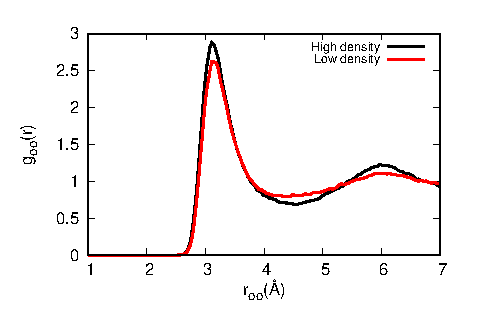
\includegraphics[width=0.45\textwidth]{cp_rdf}
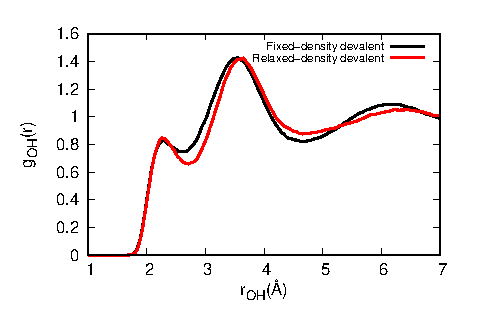
\includegraphics[width=0.45\textwidth]{cp_oh_rdf}
\caption{Oxygen-oxygen and oxygen-hydrogen radial distribution functions for the fixed-density and relaxed-density systems.}\label{Fig:rdf_cp}
\end{figure} 

In order to study the effect of intermolecular covalency on the density of liquid water, NPT-ensemble simulations were performed at 1~atm and 298~K with intermolecular charge transfer switched off. The average density of this system was determined to be 0.85~g$\cdot$cm$^{-3}$. 
This system is denoted the \emph{relaxed-density} devalent system, and contrasted with the \emph{fixed-density} devalent system used throughout the article. 

The oxygen-oxygen and oxygen-hydrogen radial distribution functions for the fixed-density and relaxed-density systems are shown in Figure~\ref{Fig:rdf_cp} for comparison. 
The positions of the peaks do not change significantly and the peaks become less pronounced after density relaxation.

\begin{figure}
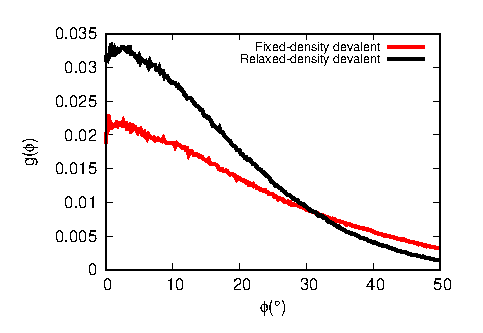
\includegraphics[width=0.45\textwidth]{cp_adf}
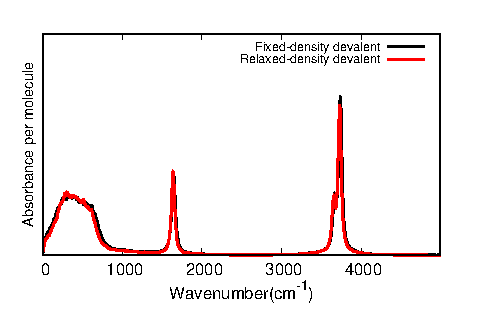
\includegraphics[width=0.45\textwidth]{cp_ir}
\caption{Angular distribution function and IR spectra for the fixed-density and relaxed-density systems.}\label{Fig:ir_cp}
\end{figure} 

Although the changes in the angular distribution functions are not significant either (Figure~\ref{Fig:ir_cp}), the distribution of HB angles becomes narrower in the relaxed-density system. The IR spectra of the two systems are almost identical (Figure~\ref{Fig:ir_cp}).

%\begin{figure}
%\caption{Angular distribution function for the 2 systems.}\label{Fig:adfcp}
%\end{figure} 
%
%\begin{figure}
%\caption{IR spectrum for the 2 systems.}\label{Fig:ir_cp}
%\end{figure} 

\section{Calculation of the HB lifetime} 

The continuous HB time-correlation function $C_{\text{HB}}(\tau)$ is defined as 
%
\bea
C_{\text{HB}}(\tau) = \frac{\sum_{ij}\langle \theta_{ij}(\tau)\theta_{ij}(0) \rangle}{\sum_{ij}\langle \theta_{ij}(0) \theta_{ij}(0) \rangle} \label{Eq:HBdecay},
\eea
%
where the HB survival function $\theta_{ij}(\tau)$ is equal to 1 if there is a HB formed between molecules $i$ and $j$ \emph{throughout} the time period from $t=0$ to $t=\tau$ and is otherwise equal to zero~\cite{rapaport1983hydrogen,starr1999fast}. 
In the long-time limit, the time-correlation function decays exponentially as shown in Fig~\ref{Fig:HBdecay}. 
The HB lifetime is defined as the rate of its decay $C_{\text{HB}}(\tau) \sim e^{-\tau/\tau_{\text{HB}}}$ and is computed as the slope of the logarithm of $C_{\text{HB}}(\tau)$.


\begin{figure}
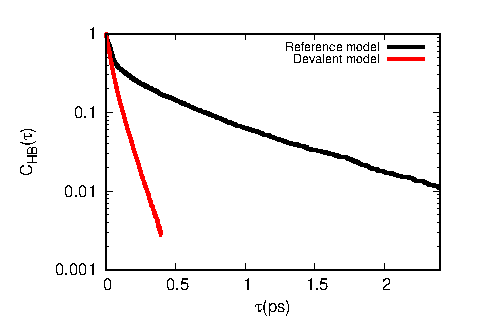
\includegraphics[width=0.4\textwidth]{new_hbdecay}
\caption{HB time autocorrelation function for the reference and devalent systems.} \label{Fig:HBdecay}
\end{figure}

\section{Calculation of the self-diffusion coefficient and shear viscosity} 

The diffusion constant for a periodic system is known to have strong dependence on the size of the simulation box $L$, due to the long-range drag exerted on a particle by its periodic images~\cite{dunweg1993molecular}. 
Fortunately, the diffusion constant in the infinitely large simulation box $D(\infty)$ can be estimated from several finite-size simulations using the following well-known relation~\cite{dunweg1993molecular}:
%
\bea
D(\infty) = D(L) + \frac{k_BT\zeta}{6\pi \eta L},
\eea
%
where $D(L)$ is the diffusion constant for a system of size $L$, $\eta$ is the translational shear viscosity, and $\zeta$ is a constant of 2.837. 
We calculated the diffusion constant $D(\infty)$ using least squares fitting to the data obtained for systems of 64, 125, and 256 molecules (Figure~\ref{Fig:dfs}). The viscosity is obtained via the slope of the $D(L)$ dependence on $1/L$.

\begin{figure}
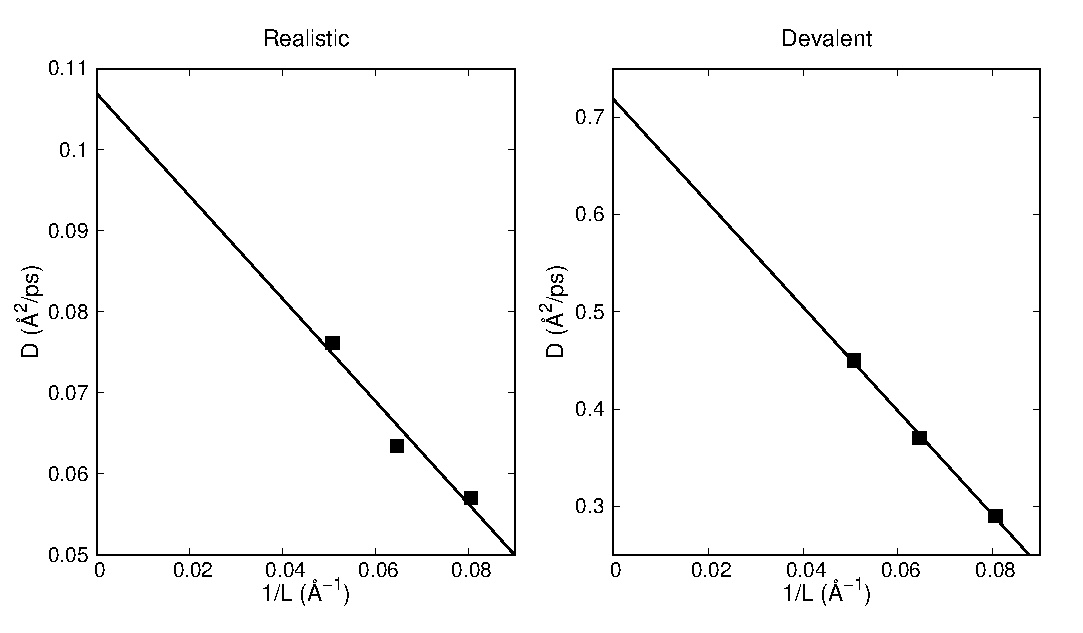
\includegraphics[width=0.47\textwidth]{msd}
\caption{Diffusion constant as a function of the system size, for 64, 125 and 256 water molecules. 
The square dots are from simulation and the solid line is a linear fit.}\label{Fig:dfs}
\end{figure} 

\section{Basis set dependence of the results} 

\begin{figure}
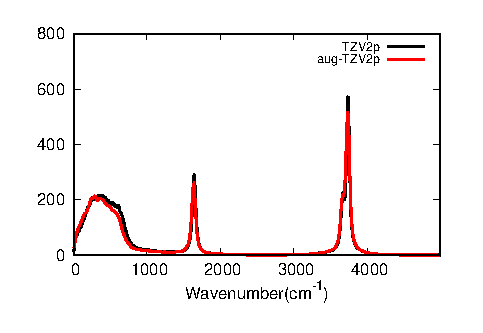
\includegraphics[width=0.45\textwidth]{basis_ir}
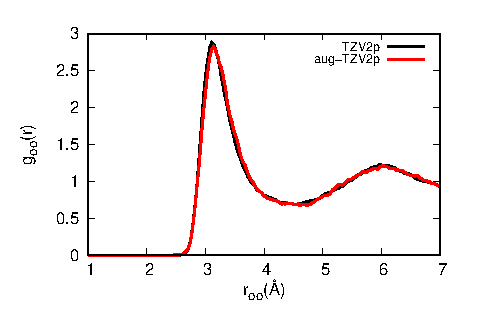
\includegraphics[width=0.45\textwidth]{basis_rdf}
\caption{IR spectra and oxygen-oxygen radial distribution functions calculated with TZV2P and aug-TZV2P basis sets.}\label{Fig:basis}
\end{figure} 

As indicated in the Computational Methods section, the accurate separation of donor-acceptor interactions from polarization effects is verified by performing simulations with two Gaussian basis sets of different sizes. 
To make the test stringent, the TZV2P basis set was extended by adding a set of diffuse functions with small exponents. 
The results of both simulations shown in Figure~\ref{Fig:basis} are practically identical. 
This indicates that TZV2P results are sufficiently stable with respect to a moderate increase in the basis set size. 
For larger basis sets, the role of intermolecular covalency will be spuriously decreased.

\fi % maintext - SI switch

\end{document}
